\pdfoutput=1
\documentclass[11pt]{article}
\usepackage{eacl2023}
\usepackage{times}
\usepackage{latexsym}
\usepackage[T1]{fontenc}
\usepackage[utf8]{inputenc}
\usepackage{microtype}
\usepackage{graphicx}
\usepackage{booktabs}
\usepackage{url}
\usepackage{placeins}
\usepackage{array}

\title{Bias-Aware Indic Spoken Language Identification:\\Task 1-3 Report}

\author{Project Team \\
Saarland University \\
\texttt{spoken-language-identification}}

\begin{document}
\maketitle

\begin{abstract}
This report covers all three project tasks for Indic spoken language identification on \texttt{badrex/nnti-dataset-full}. In Task 1, we reproduced baseline pipelines and compared pretrained backbones. In Task 2, we addressed speaker shortcut bias through data-centric augmentation and model-based adversarial training (DANN). In Task 3, we analyzed likely bias sources, confusion patterns, and representation behavior with t-SNE. Across complete runs, the strongest model in our branch is DANN over mHuBERT, improving validation accuracy from 0.4676 (untuned mHuBERT baseline) to 0.5576 and macro-F1 from 0.4142 to 0.5426 while preserving speaker-disjoint validation integrity.
\end{abstract}

\section{Introduction}
Spoken language identification (SLID) in low-resource, multi-speaker settings is vulnerable to shortcut learning: models may rely on speaker identity cues instead of language-specific cues. Our project is organized into three tasks: (1) reproduce and improve baseline performance, (2) mitigate speaker bias, and (3) analyze outcomes with quantitative diagnostics and visualization.

Our implementation is based on PyTorch \citep{paszke2019pytorch} and Hugging Face Transformers/Datasets \citep{wolf2020transformers}. For analysis tooling, we used scikit-learn \citep{pedregosa2011scikit} and Matplotlib \citep{hunter2007matplotlib}. We evaluated pretrained speech encoders including MMS \citep{pratap2023mms}, wav2vec 2.0 \citep{baevski2020wav2vec2}, and mHuBERT (HuBERT family \citep{hsu2021hubert}).

\section{Data and Experimental Protocol}
We use \texttt{badrex/nnti-dataset-full} \citep{badr2026dataset}, which provides predefined \texttt{train}/\texttt{validation} splits.

Key characteristics from diagnostics:
\begin{itemize}
    \item 22 target languages.
    \item 8689 train samples, 3300 validation samples.
    \item 110 unique train speakers.
    \item 681 unique validation speakers.
    \item Speaker overlap between train and validation: 0.
\end{itemize}

Model selection is based on validation metrics with best-checkpoint loading enabled. We report accuracy, macro-F1, eval loss, per-language accuracy, confusion matrices, and speaker diagnostics.

\subsection{Methods and Experimental Settings}
To keep comparisons fair across Task 1/2/3 experiments, we kept the split protocol fixed and changed only the intended method components. Core controls were: fixed seed (42), same dataset split, same base backbone family (mHuBERT for final comparisons), and best-checkpoint selection rather than last-step reporting.

Task 1 experiments compare pretrained backbones and then a tuned mHuBERT reference. Task 2 experiments start from the tuned no-mitigation reference and introduce either (i) data-centric augmentation or (ii) adversarial speaker de-biasing. Task 3 uses run artifacts (metrics, confusion, speaker diagnostics, t-SNE outputs) for evidence-based analysis.

\section{Task 1: Baseline Recreation and Improvement}
\subsection{Models and Results}
Table~\ref{tab:task1-models} summarizes major Task 1 runs (validation split).

\begin{table}[t]
\centering
\small
\begin{tabular}{lccc}
\toprule
Model / Run & Accuracy & Macro-F1 & Eval Loss \\
\midrule
facebook-mms-300m & 0.2197 & 0.1892 & 2.7230 \\
wav2vec2-xls-r-300m & 0.0900 & 0.0486 & 3.0646 \\
mHuBERT (untuned) & 0.4676 & 0.4142 & 2.2854 \\
mHuBERT (tuned) & 0.5270 & 0.4748 & 2.1629 \\
\bottomrule
\end{tabular}
\caption{Task 1 validation performance across backbone choices and tuning.}
\label{tab:task1-models}
\end{table}

\subsection{Task 1 Conclusion}
In our environment, mHuBERT with tuning is the strongest Task 1 setting, improving over untuned mHuBERT by +0.0594 accuracy and +0.0607 macro-F1. We use this tuned run as the no-mitigation reference for Task 2.

\section{Task 2: Speaker-Bias Mitigation}
\subsection{Problem and Approaches}
With limited speaker diversity per language in training, the model can reduce loss by exploiting speaker-correlated signals, creating a clear shortcut risk.

We evaluated:
\begin{itemize}
    \item Data-centric mitigation (train-only augmentation): speed perturbation + waveform noise (Mitigation 1).
    \item Model-based mitigation: DANN with gradient reversal \citep{ganin2016dann}.
    \item Intermediate ablations (Mitigation 2, 3A, 3B, 4) to study tradeoffs.
\end{itemize}

\paragraph{Method details.}
For data-centric mitigation, augmentation is applied only on train samples (not validation), with probabilistic speed/noise perturbation. For model-based mitigation, DANN uses a shared encoder with a language head and an adversarial speaker head through gradient reversal.

At encoder level, the optimization target is:
\[
\mathcal{L}_{enc} = \mathcal{L}_{lang} - \lambda \mathcal{L}_{speaker}
\]
which encourages language-discriminative but speaker-invariant features. In our final DANN run, we used \texttt{speaker\_loss\_weight}=0.1 and \texttt{grl\_lambda}=1.0 with scheduling.

\subsection{Mitigation Results}
\begin{table}[t]
\centering
\small
\setlength{\tabcolsep}{2.5pt}
\begin{tabular}{@{}p{0.47\columnwidth}rrr@{}}
\toprule
Run & Acc & Macro-F1 & Loss \\
\midrule
Tuned ref (no mitigation) & 0.527 & 0.475 & 2.163 \\
Mitigation 1 (data-centric) & 0.539 & 0.487 & 2.150 \\
Mitigation 2 & 0.528 & 0.483 & 2.139 \\
Mitigation 3A & 0.498 & 0.456 & 2.188 \\
Mitigation 3B & 0.528 & 0.482 & 2.146 \\
Mitigation 4 & 0.512 & 0.466 & 2.213 \\
DANN (final improved) & \textbf{0.558} & \textbf{0.543} & \textbf{1.881} \\
\bottomrule
\end{tabular}
\caption{Task 2 mitigation results (validation split).}
\label{tab:task2-mitigation}
\end{table}

\subsection{Extent of Success}
Relative to untuned baseline mHuBERT, DANN improves by +0.0900 accuracy and +0.1284 macro-F1. Relative to Mitigation 1, DANN still improves by +0.0188 accuracy and +0.0558 macro-F1.

Speaker-oriented evidence:
\begin{itemize}
    \item Unseen-speaker validation accuracy: 0.4676 (untuned) $\rightarrow$ 0.5576 (DANN).
    \item Train/validation speaker overlap remains 0 (no leakage warning).
    \item Key bias-sensitive confusions reduced, e.g., \texttt{sindhi$\rightarrow$punjabi}: 79 $\rightarrow$ 14.
\end{itemize}

These results indicate meaningful mitigation of speaker-related shortcuts, but not complete removal of speaker information.

\subsection{Ablation and Efficiency Summary}
To make the mitigation decision explicit, Table~\ref{tab:ablation-efficiency} reports deltas relative to the tuned no-mitigation reference.

\begin{table}[t]
\centering
\small
\setlength{\tabcolsep}{2.5pt}
\begin{tabular}{@{}p{0.46\columnwidth}rrr@{}}
\toprule
Run & $\Delta$Acc & $\Delta$F1 & Train hrs \\
\midrule
Tuned ref (no mitigation) & 0.000 & 0.000 & 5.51 \\
Mitigation 1 & +0.012 & +0.012 & 6.65 \\
Mitigation 2 & +0.001 & +0.008 & 6.17 \\
Mitigation 3A & -0.029 & -0.019 & 9.24 \\
Mitigation 3B & +0.001 & +0.007 & 9.18 \\
Mitigation 4 & -0.015 & -0.008 & 5.99 \\
DANN (final improved) & \textbf{+0.031} & \textbf{+0.068} & 8.18 \\
\bottomrule
\end{tabular}
\caption{Ablation summary relative to tuned reference.}
\label{tab:ablation-efficiency}
\end{table}

Interpretation: Mitigation 1 gives a stable data-centric gain; Mitigation 2 and 3B are near-tied but below Mitigation 1; Mitigation 3A regresses; Mitigation 4 underperforms Mitigation 1; DANN provides the strongest final improvement, with higher training cost but a better accuracy/F1 tradeoff.

\section{Task 3: Analysis}
\subsection{Source of Bias and Learning Difficulty}
The data regime (few train speakers per language, fully unseen validation speakers) creates strong shortcut pressure. Early optimization may latch onto speaker timbre/prosody, while weaker classes remain under-separated. This pattern appears in near-zero class performance for the untuned baseline (e.g., maithili, konkani) and concentrated confusion clusters.

\subsection{Confusion Analysis}
Most frequent confusions include:
\begin{itemize}
    \item \texttt{konkani$\rightarrow$marathi}
    \item \texttt{sindhi$\rightarrow$punjabi}
    \item \texttt{hindi$\rightarrow$urdu}
\end{itemize}
Likely drivers include linguistic/acoustic proximity and imbalance in class difficulty. DANN reduces several dominant pairs but does not eliminate all structural confusion.

\begin{table}[t]
\centering
\small
\setlength{\tabcolsep}{3pt}
\begin{tabular}{@{}p{0.48\columnwidth}rrr@{}}
\toprule
Pair (true$\rightarrow$pred) & Baseline & DANN & $\Delta$ \\
\midrule
konkani$\rightarrow$marathi & 106 & 74 & -32 \\
sindhi$\rightarrow$punjabi & 79 & 14 & -65 \\
hindi$\rightarrow$urdu & 60 & 39 & -21 \\
santali$\rightarrow$bengali & 54 & 10 & -44 \\
dogri$\rightarrow$punjabi & 53 & 44 & -9 \\
\midrule
bodo$\rightarrow$manipuri & 39 & 45 & +6 \\
\bottomrule
\end{tabular}
\caption{Confusion-pair count changes from untuned baseline to DANN. Negative $\Delta$ is an improvement (fewer errors).}
\label{tab:confusion-delta}
\end{table}

\begin{figure*}[t]
    \centering
    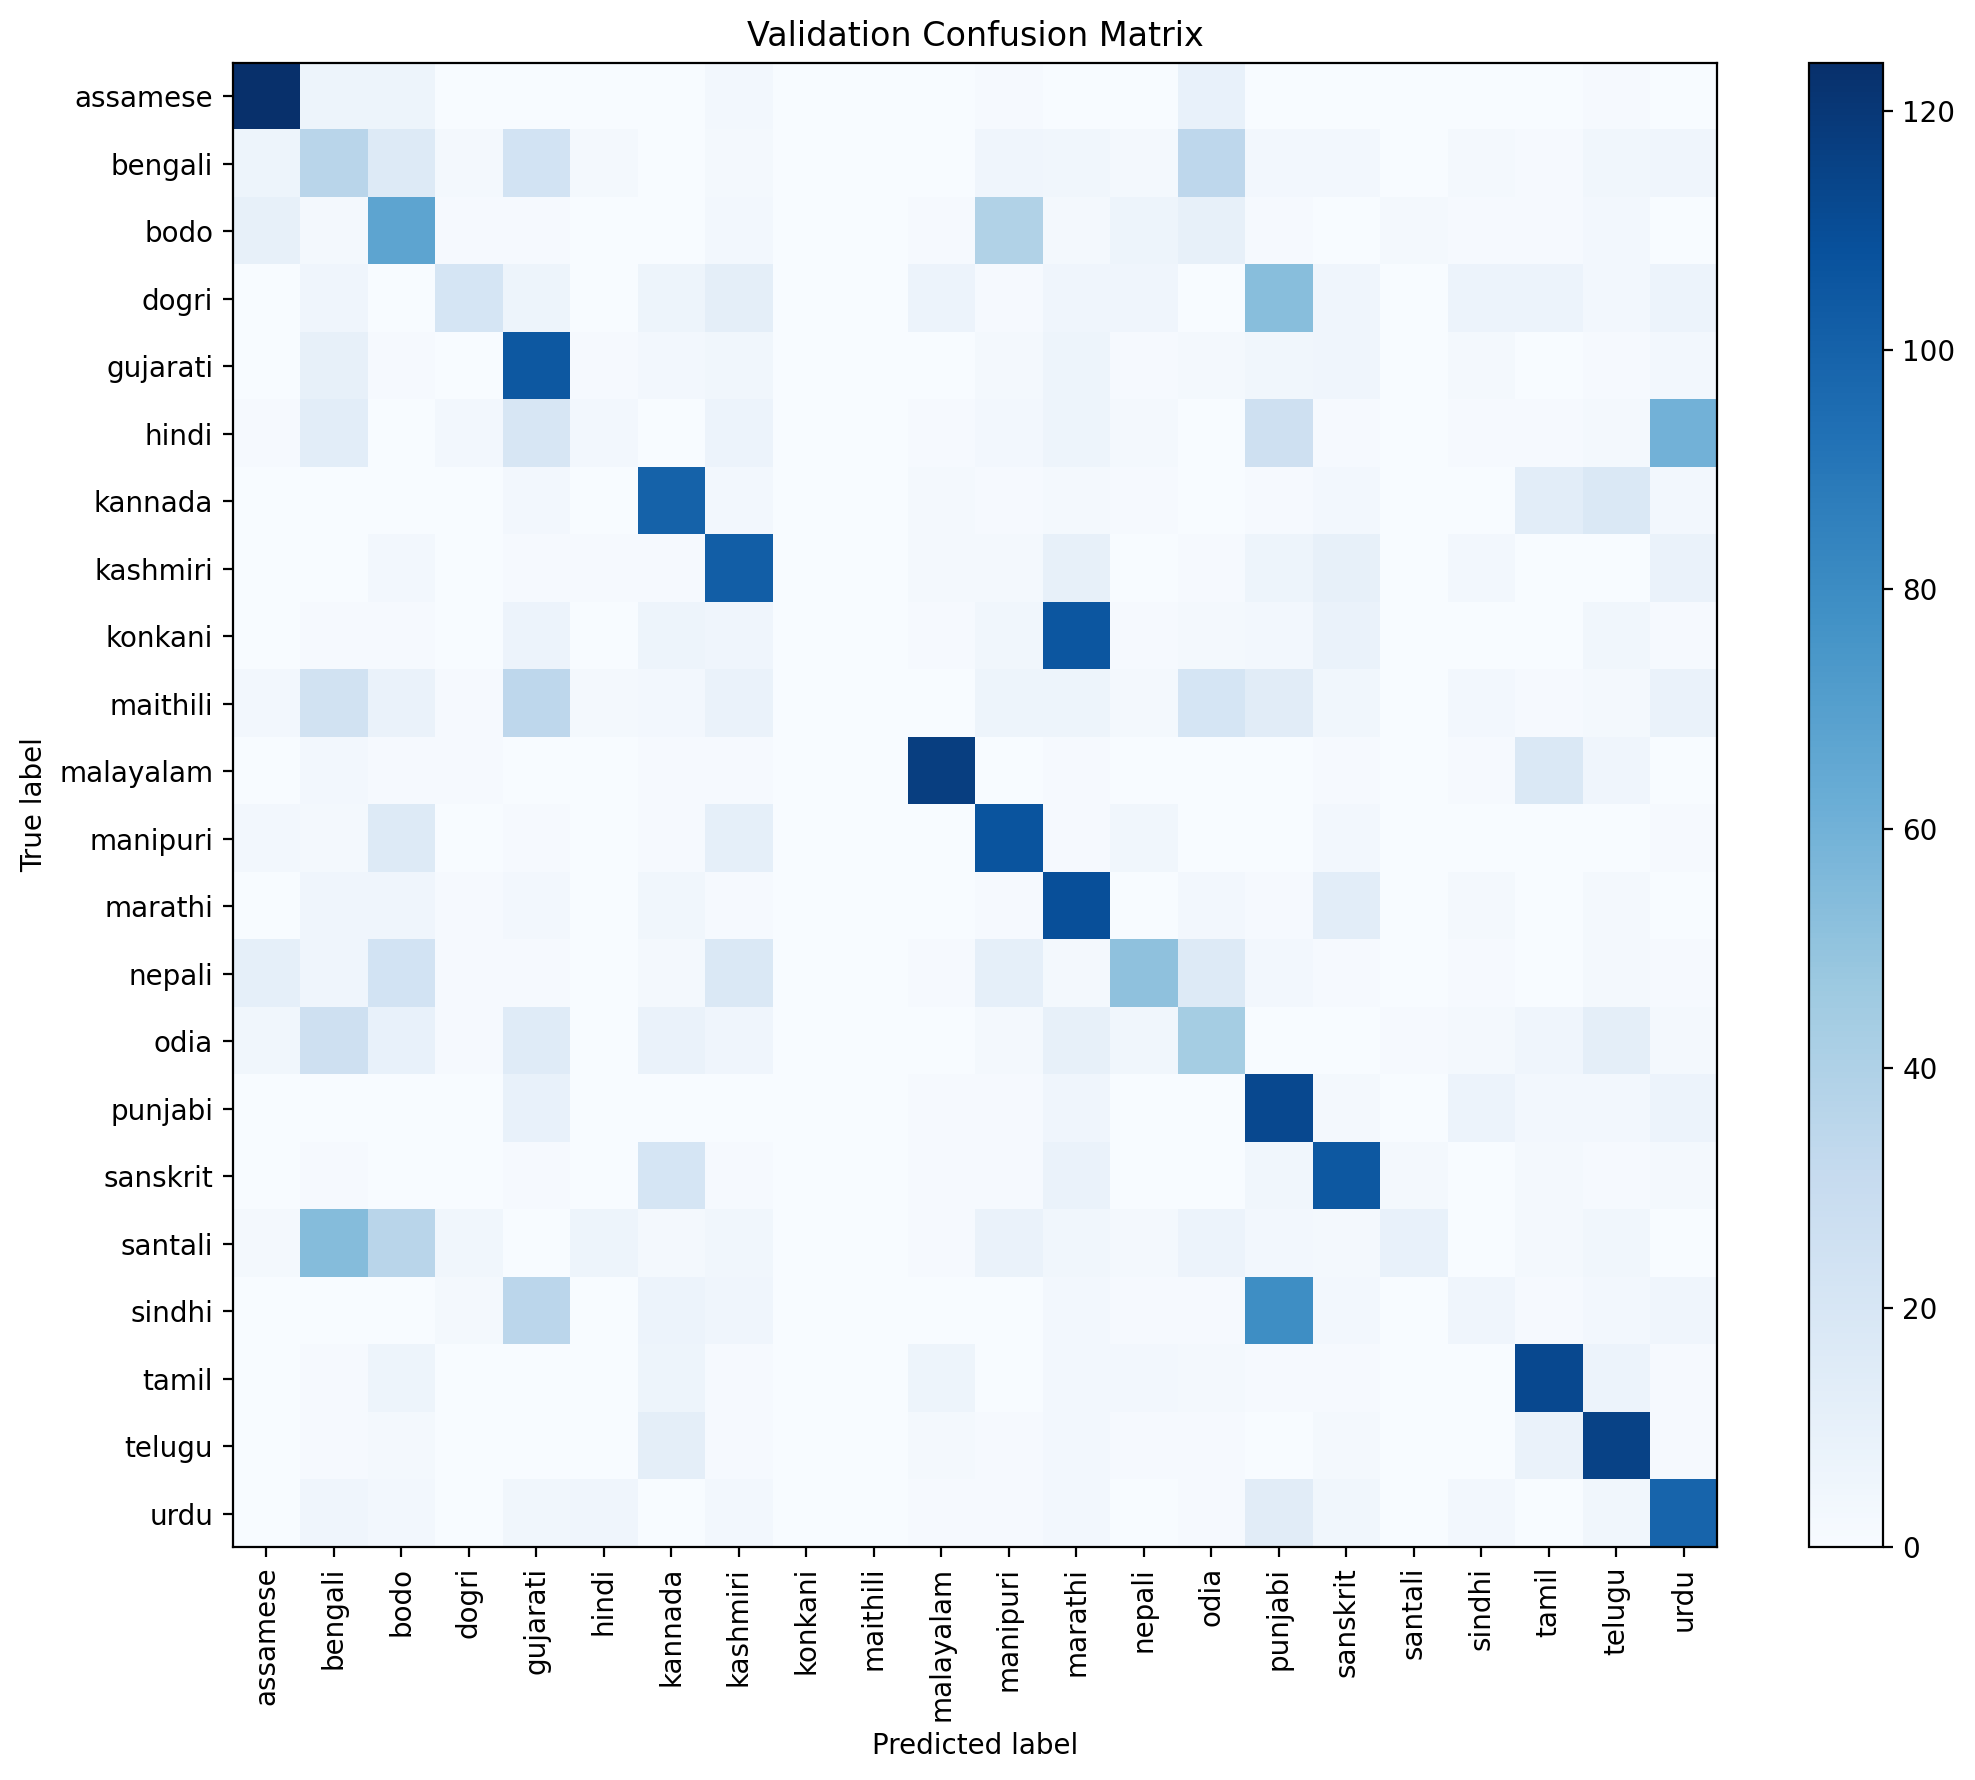
\includegraphics[width=0.31\textwidth]{assets/confusion_baseline_untuned.png}
    \hfill
    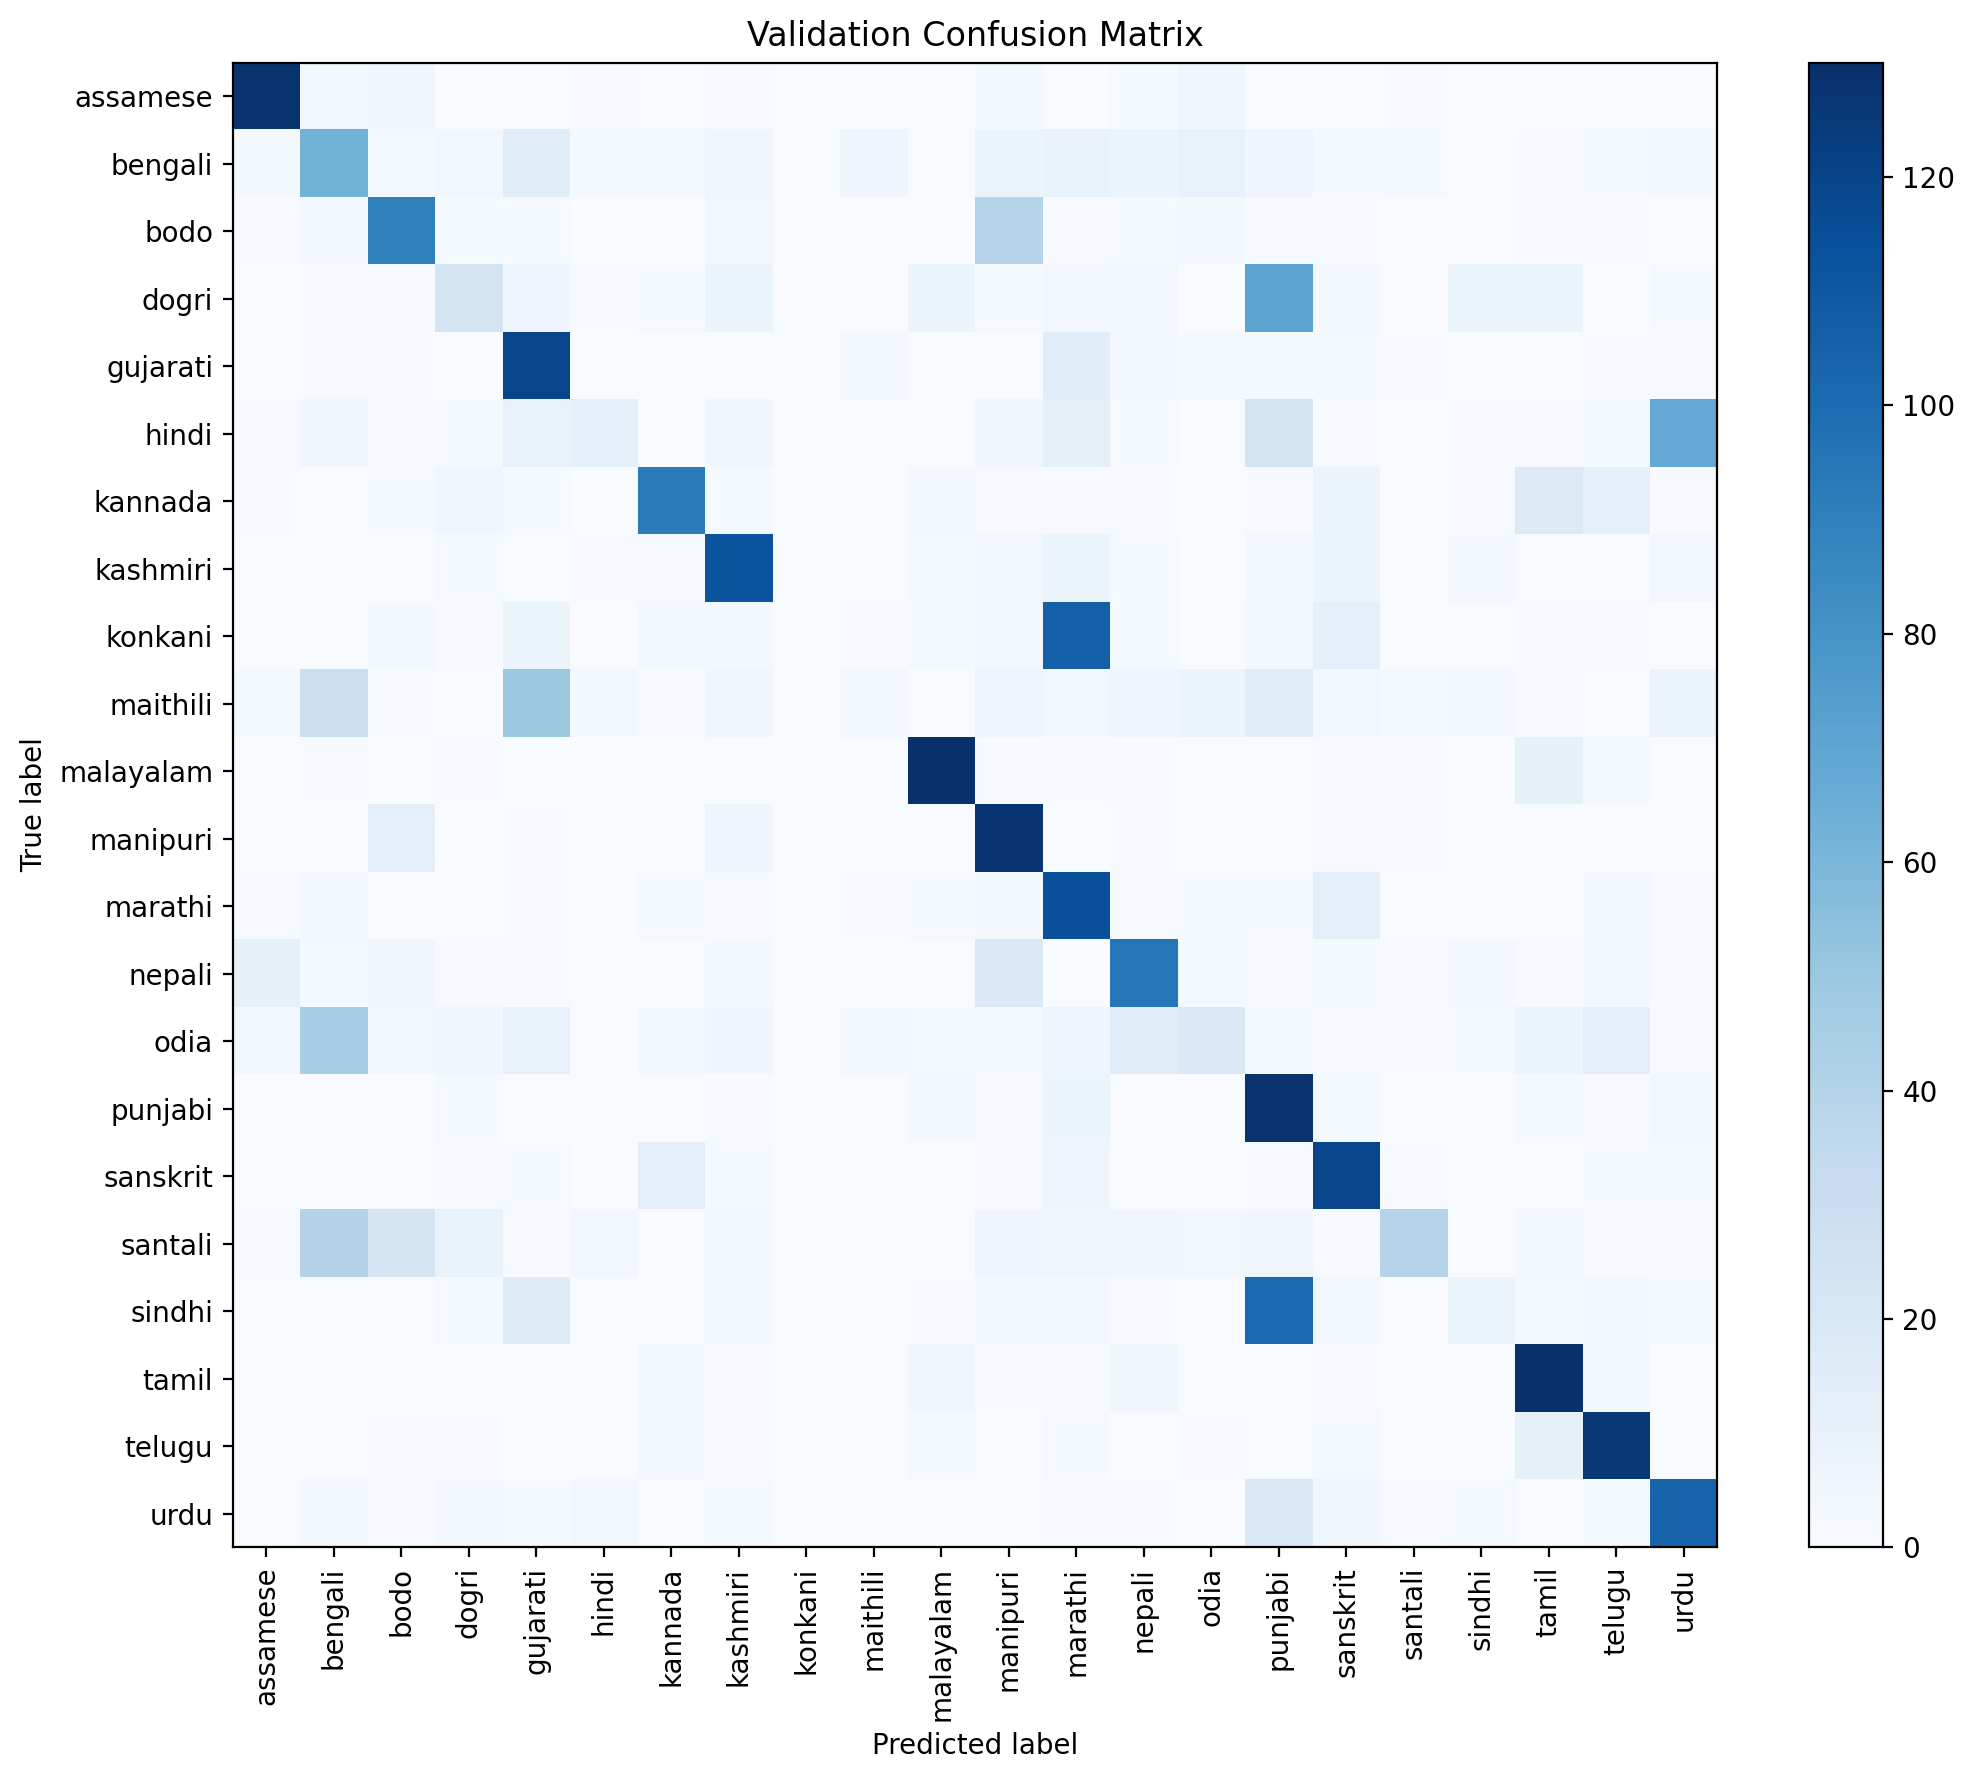
\includegraphics[width=0.31\textwidth]{assets/confusion_mitigation1.png}
    \hfill
    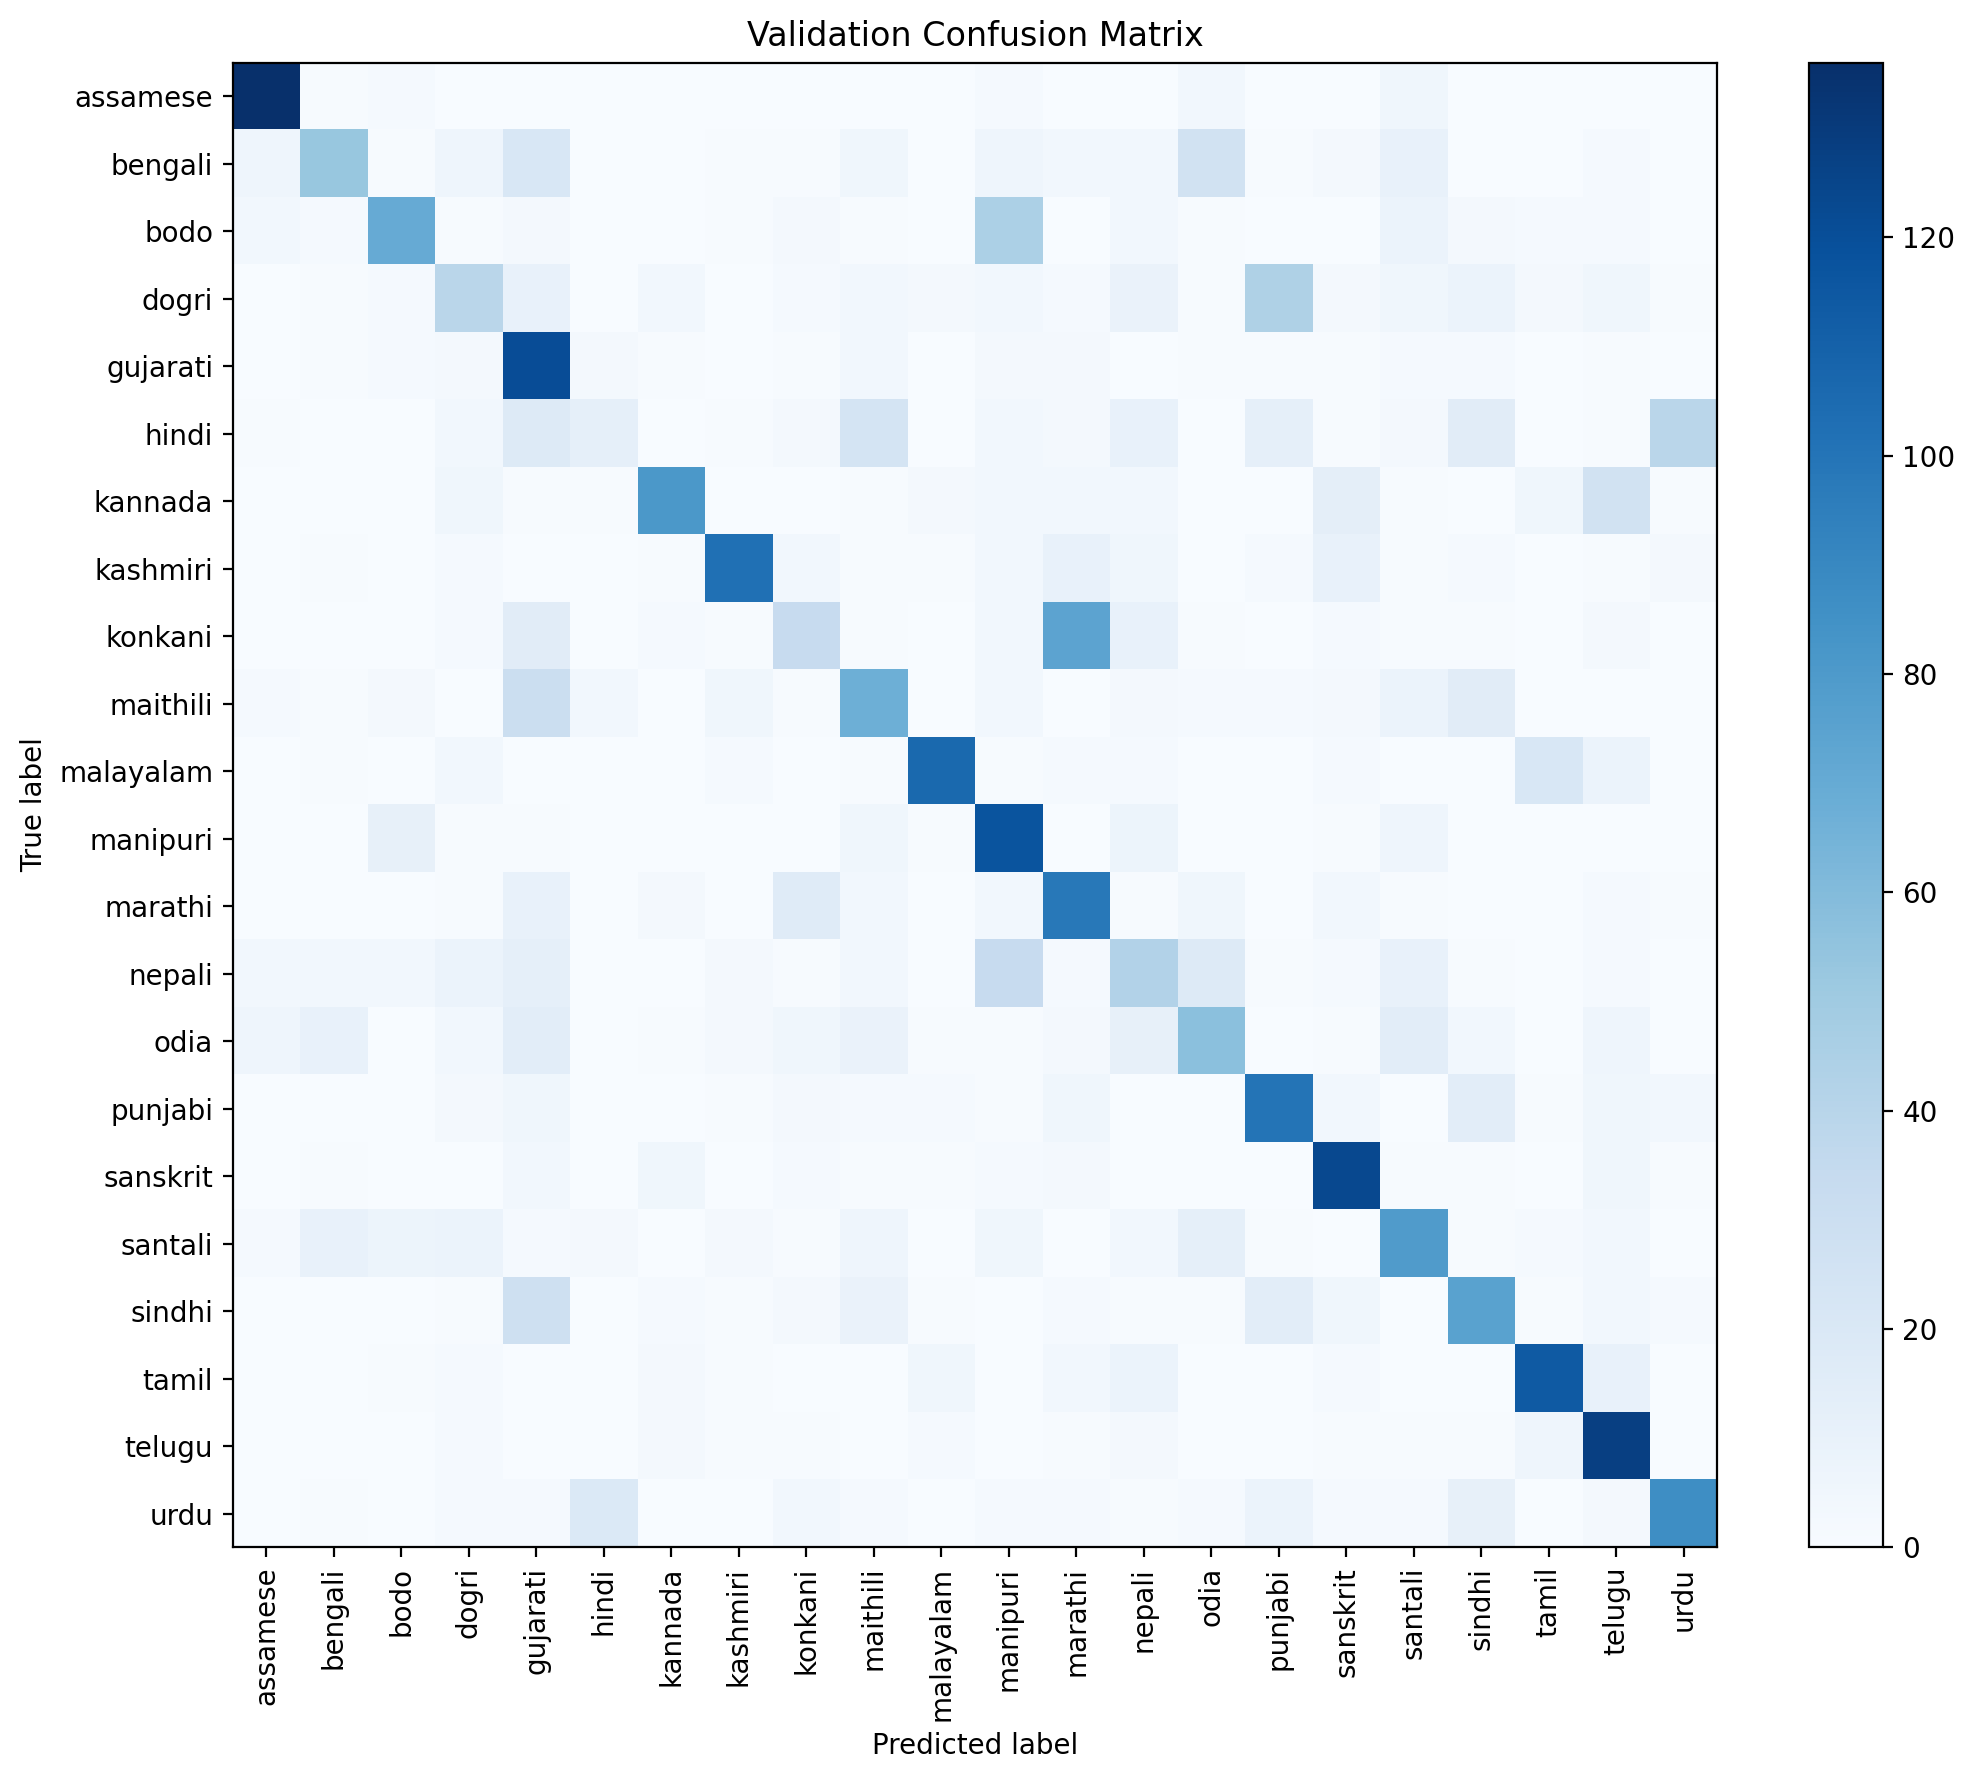
\includegraphics[width=0.31\textwidth]{assets/confusion_dann.png}
    \caption{Validation confusion matrices: untuned baseline (left), Mitigation 1 (middle), and DANN improved (right).}
    \label{fig:cm-bu-dann}
\end{figure*}

\subsection{Representation Analysis (t-SNE)}
We applied t-SNE \citep{maaten2008tsne} to last-layer validation embeddings for the improved run. Baseline/tuned/M1 t-SNE export was not reproducible from current local artifacts because those run folders do not contain full model/preprocessor checkpoint files.

For DANN:
\begin{itemize}
    \item Silhouette (language): 0.0047
    \item Silhouette (speaker top-k): -0.0992
    \item kNN speaker purity@5: 0.3433
\end{itemize}
Interpretation: speaker identity appears reduced but is still partially encoded.

\begin{figure}[t]
    \centering
    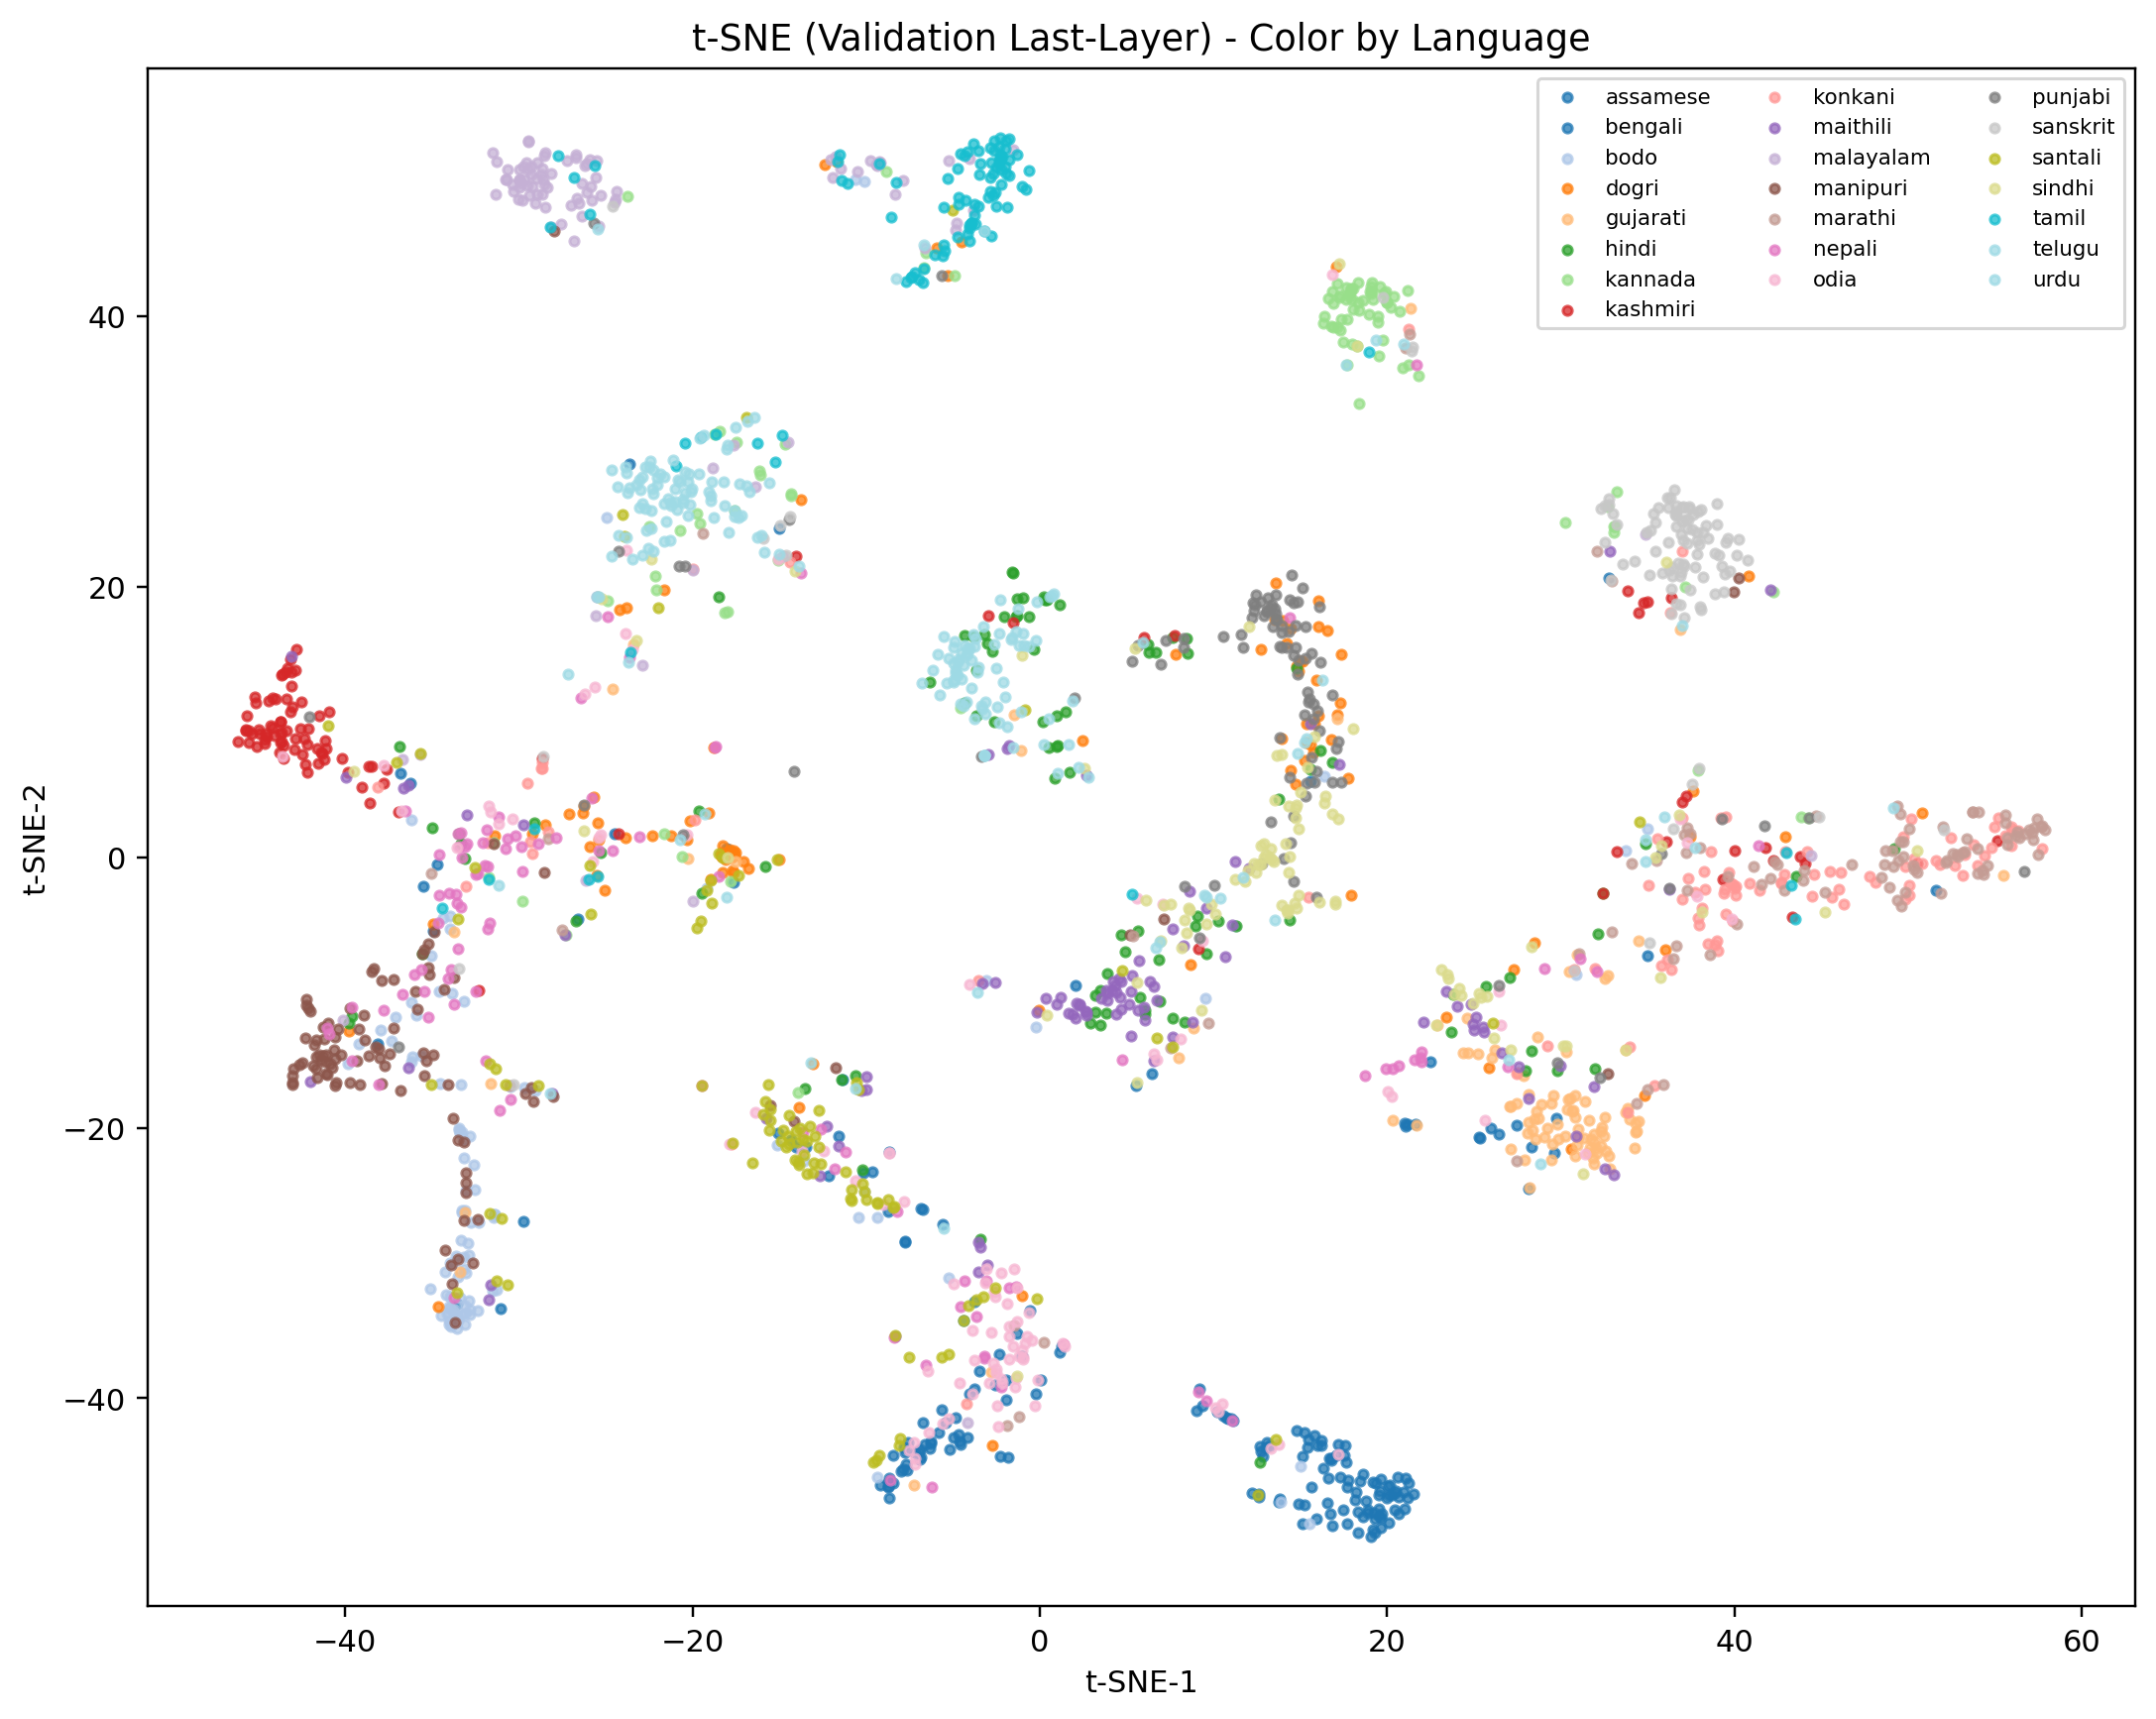
\includegraphics[width=0.48\linewidth]{assets/tsne_dann_by_language.png}
    \hfill
    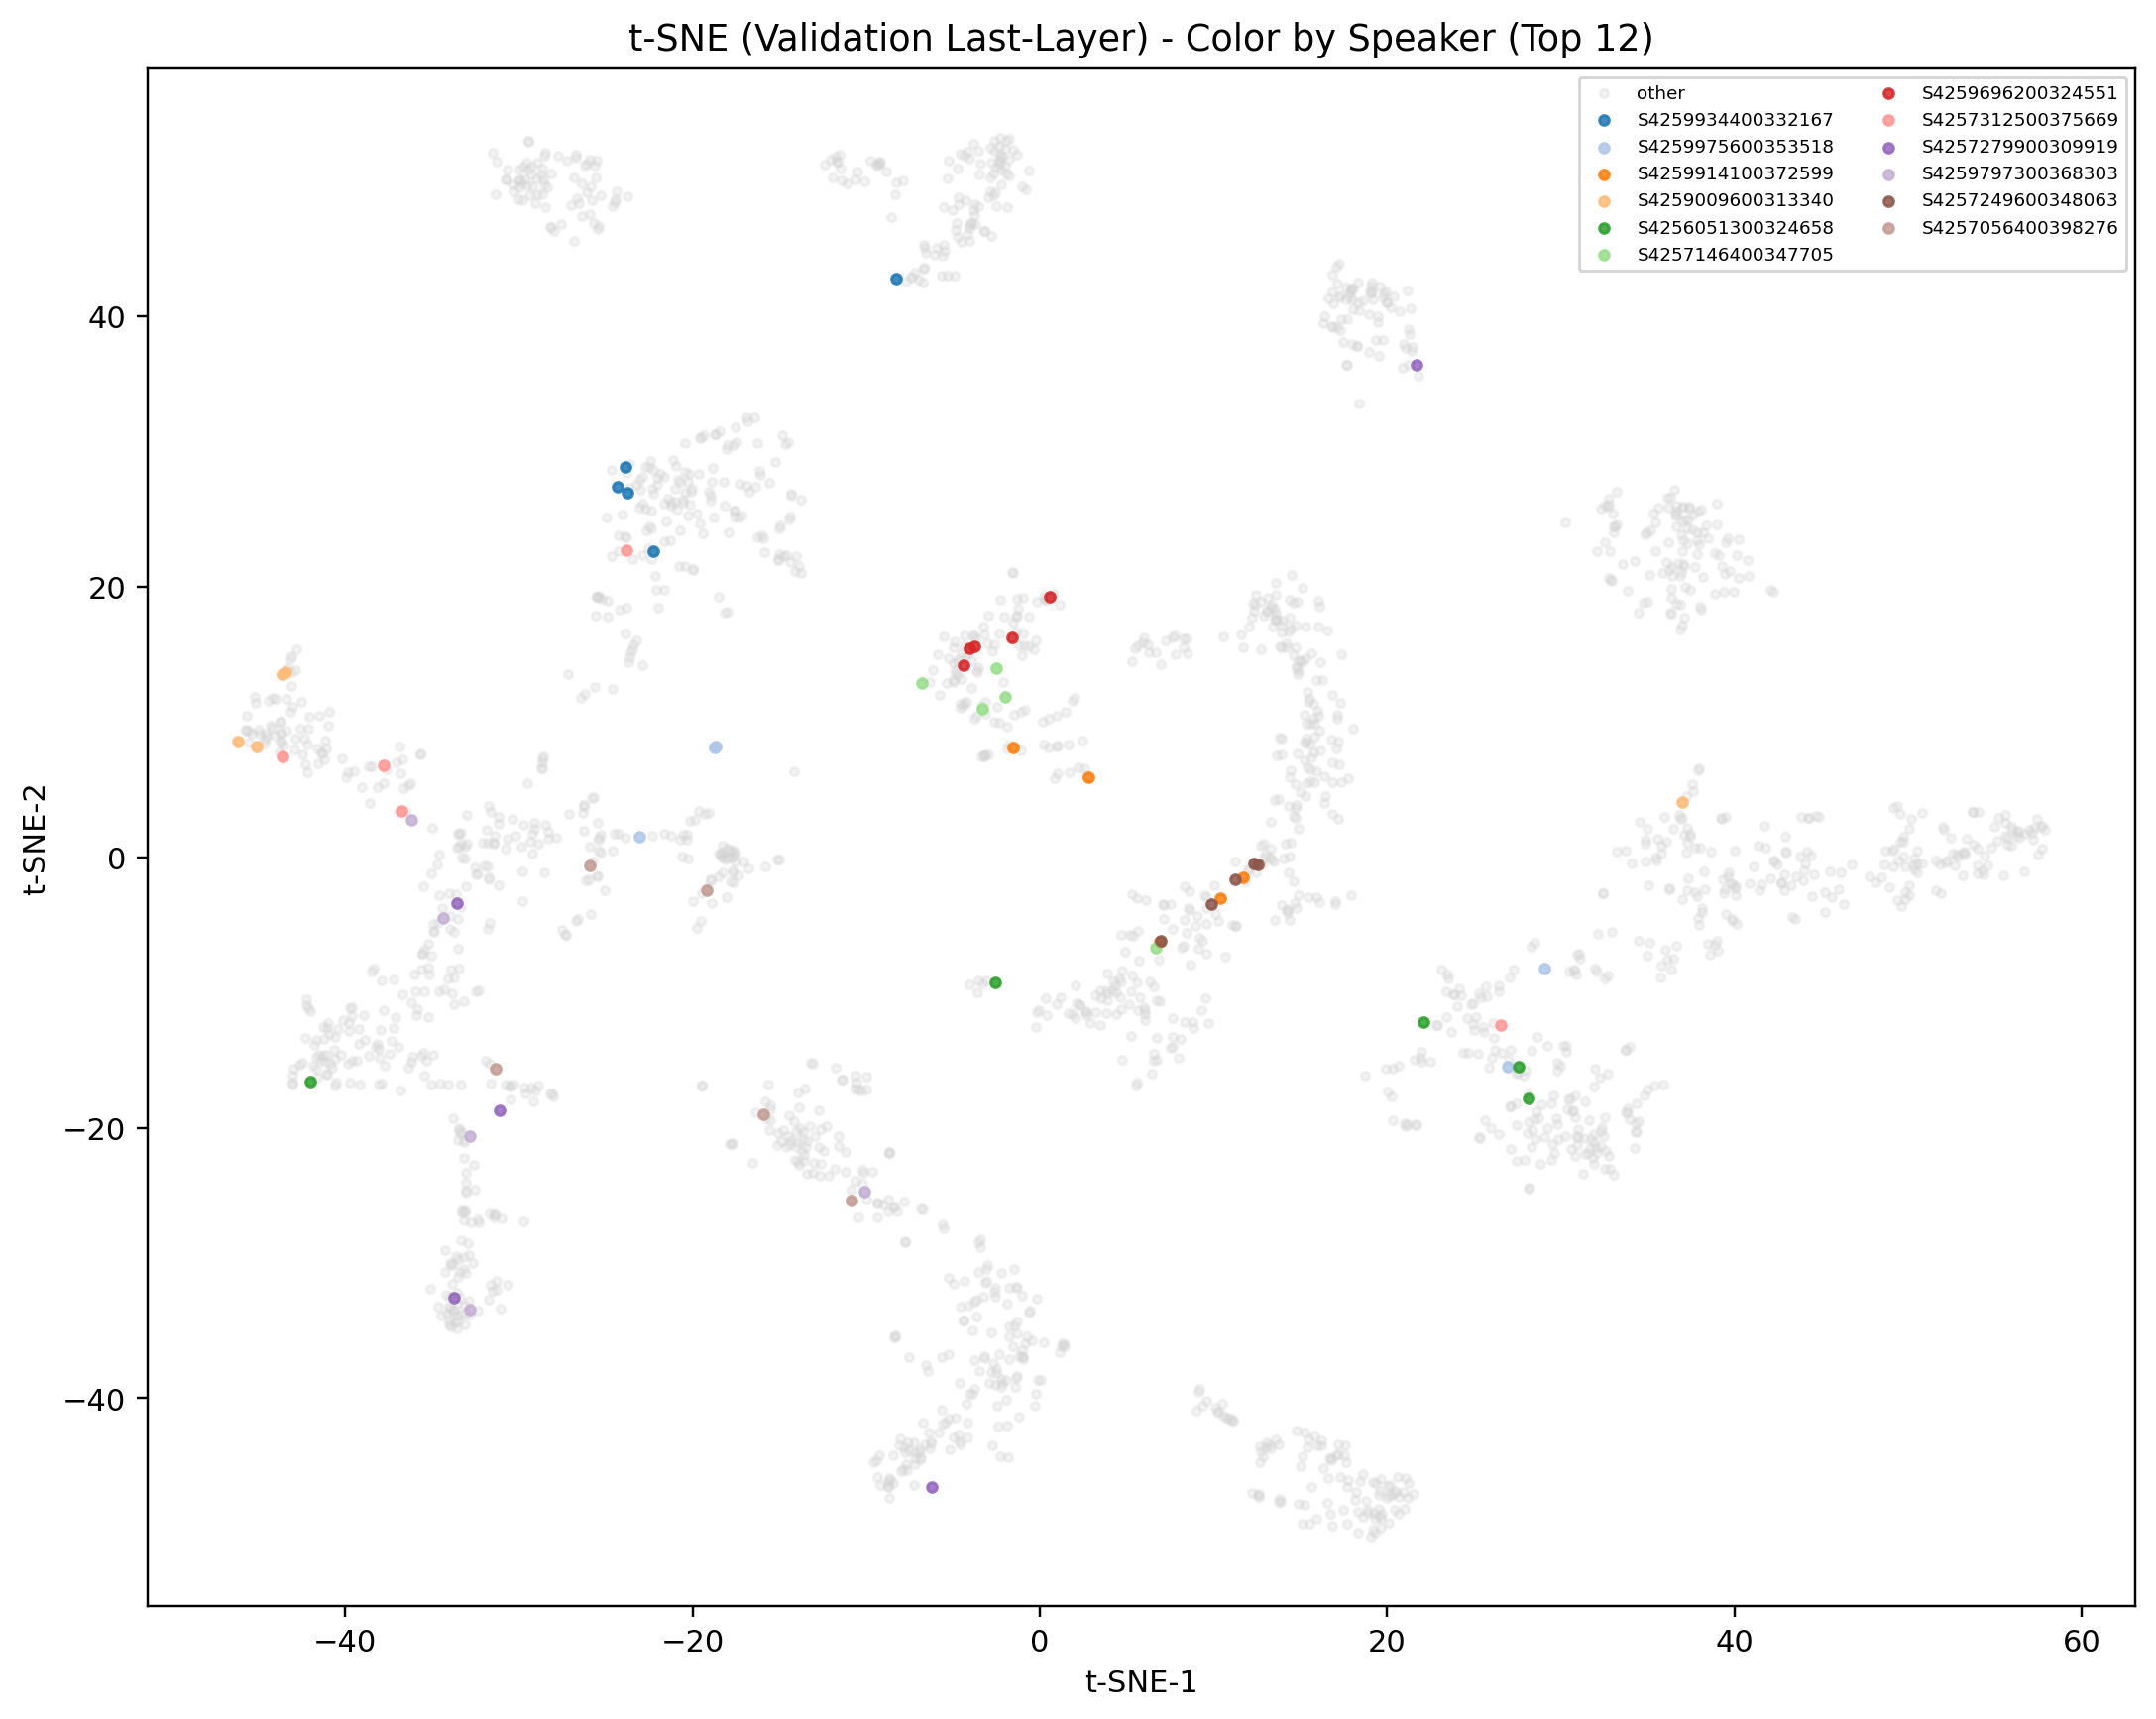
\includegraphics[width=0.48\linewidth]{assets/tsne_dann_by_speaker.png}
    \caption{DANN t-SNE on validation embeddings: language coloring (left) and speaker coloring (right).}
    \label{fig:tsne-dann}
\end{figure}

\subsection{Additional Insightful Analyses}
To avoid single-metric conclusions, we added the following quantitative analyses:
\begin{itemize}
    \item Class-balance profile across runs (mean/median/min/max per-language accuracy).
    \item Weak-class recovery index (baseline weak set: hindi, konkani, maithili, santali, sindhi).
    \item Error concentration (top-5 confusion mass ratio).
    \item Best-step ratio (best step / final step) to show late-epoch plateau and justify best-checkpoint reporting.
\end{itemize}
These analyses are documented in \texttt{reports/task3\_analysis.md} and \texttt{reports/tables/}.

\section{Reproducibility Notes}
We report the exact run IDs and artifacts used in analysis (\texttt{reports/artifacts\_used.md}). Core reproducibility settings are:
\begin{itemize}
    \item Seed: 42.
    \item Training epochs: 3.
    \item Mac profile for final mitigation runs: batch size 1, gradient accumulation 4, max duration 7\,s, max grad norm 1.0, evaluation/save every 100 steps.
    \item Best-checkpoint loading enabled; mitigation runs selected with macro-F1 criterion.
    \item Speaker diagnostics and confusion matrices generated for every final compared run.
\end{itemize}
For Mitigation 3B and Mitigation 4, summary metrics in this report are taken from archived project reports in \texttt{reports/} because the corresponding full run directories are not present in the current branch snapshot.
These controls reduce accidental variance and support a fair mitigation comparison.

\FloatBarrier

\section{Conclusion}
Across all three tasks, mHuBERT is the strongest backbone in our environment. Data-centric mitigation improves balanced performance, and DANN yields the best final model. The final DANN run achieves 0.5576 validation accuracy and 0.5426 macro-F1 with clean speaker-disjoint diagnostics. Remaining challenges are concentrated in a small set of linguistically close language pairs.

\section*{Limitations}
First, the strongest t-SNE comparison currently uses improved-run embeddings, while baseline/tuned/M1 t-SNE export is limited by missing checkpoint artifacts in those run folders. Second, some persistent confusions (e.g., konkani-marathi) remain unresolved and may require additional data balancing or task-specific objectives. Third, compute constraints limit the number of long-run and combined-mitigation experiments.

\section*{Ethics Statement}
This work focuses on technical mitigation of dataset bias and does not deploy a user-facing system. We explicitly monitored speaker overlap and unseen-speaker behavior to reduce leakage-driven claims. Because language recognition systems can be misused for profiling, we report calibrated conclusions and avoid claims of complete bias removal.

\FloatBarrier
\bibliographystyle{acl_natbib}
\bibliography{custom}

\end{document}
